%#########################################################################
\chapter{Ondas Elásticas}
\label{cha:waves}


%#########################################################################



\
%*************************************************************************
\section{Demostración 1: Ondas en una Membrana Circular}
\label{sec:DEMO3_01}
\rule{14cm}{0.5mm}

Como primer caso se aborda el péndulo simple. Este consiste en un sistema
de una masa $m$ con dimensión despreciable y bajo la acción de la 
gravedad $\bds g$, además pende de una cuerda tensa de longitud $l$ y sujeta
en un punto fijo. A partir de la figura \ref{fig:simple_pendulum}, la 
ecuación de movimiento está dada por


%.........................................................................
%Movement equation
\eq{eq:simple_pendulum}
{m\dtot{^2\bds r}{t^2} = m\bds g + \bds T}
%.........................................................................

\newpage
%.........................................................................
%Simple Pendulum
\begin{figure}[htbp]
	\centering
	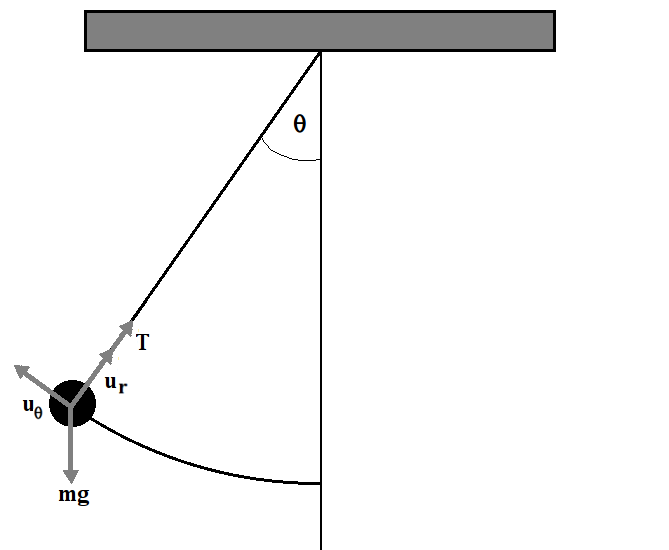
\includegraphics[width=0.80\textwidth]
	{./pictures/simple_pendulum.png}

	\caption{\small{Péndulo simple bajo la acción del campo gravitacional.}}
	
	\label{fig:simple_pendulum}
\end{figure}
%.........................................................................


\newpage
%ccccccccccccccccccccccccccccccccccccccccccccccccccccccccccccccccccccccccc
%DEMO 2_01
\begin{listing}[style=python]
#!/usr/bin/env python
#==========================================================
# DEMOSTRACION 1
# Grafica de soluciones aproximadas del pendulo simple
#==========================================================
import numpy as np
import matplotlib.pylab as plt

#Solucion
def Theta(t):
    theta = theta0*np.sin( omega0*t + delta )
    return theta
    
#Gravedad
g = 9.8
#Longitud
l = 1
#Frecuencia
omega0 = np.sqrt( g/l )
#Tiempos
tiempo = np.arange( 0, 10, 0.1 )
    
#SOLUCION 1
#Amplitud
theta0 = 0.05
#Fase
delta = 0.0
#Grafica
plt.plot( tiempo, Theta(tiempo), label='solucion 1' )

#SOLUCION 2
#Amplitud
theta0 = 0.05
#Fase
delta = np.pi
#Grafica
plt.plot( tiempo, Theta(tiempo), label='solucion 2' )

#SOLUCION 3
#Amplitud
theta0 = 0.1
#Fase
delta = 0.0
#Grafica
plt.plot( tiempo, Theta(tiempo), label='solucion 3' )

plt.legend()
plt.show()
\end{listing}
%ccccccccccccccccccccccccccccccccccccccccccccccccccccccccccccccccccccccccc


%ccccccccccccccccccccccccccccccccccccccccccccccccccccccccccccccccccccccccc
%DEMO 2_01
\begin{listing}[style=python, numbers = none]
import numpy as np
import matplotlib.pylab as plt
\end{listing}
%ccccccccccccccccccccccccccccccccccccccccccccccccccccccccccccccccccccccccc

%*************************************************************************




\
%*************************************************************************
\section{Demostración 2: Efecto Doppler}
\label{sec:DEMO3_02}
\rule{14cm}{0.5mm}

El efecto doppler es un fenómeno físico que se presenta en sistemas donde
hay fuentes y observadores en movimiento relativo. En esta demostración se 
abordará el efecto dopplet acústico simulando la señal obtenida por el 
movimiento de una fuente respecto a un obsevador en reposo.

\
%.........................................................................
%Doppler effect
\begin{figure}[htbp]
	\centering
	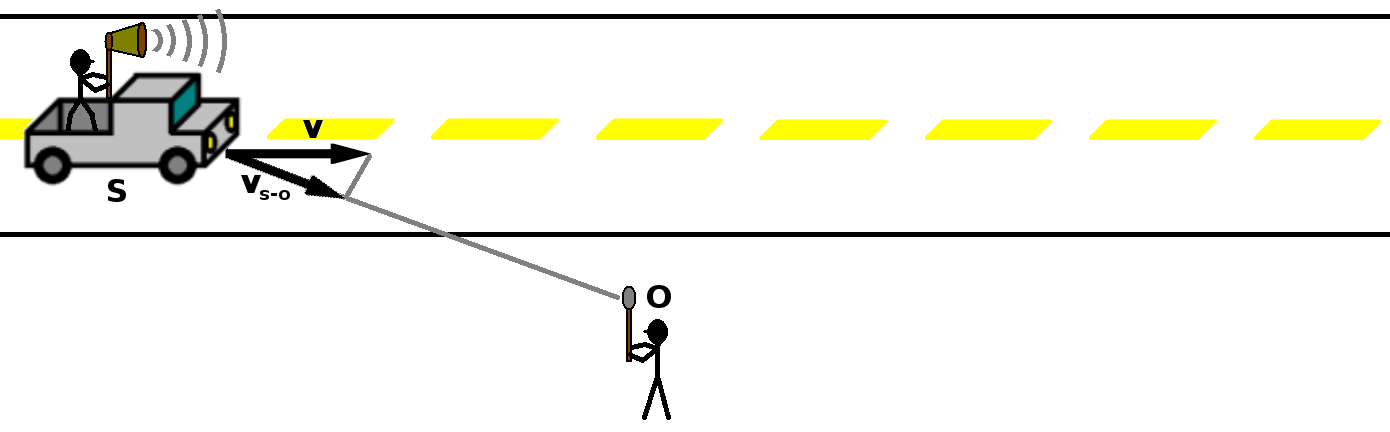
\includegraphics[width=0.90\textwidth]
	{./pictures/doppler.png}

	\caption{\small{Ilustración de efecto doppler acústico con una 
	fuente en movimiento.}}
	
	\label{fig:doppler}
\end{figure}
%.........................................................................


Por simplicidad se asumirá que la señal emitida por la fuente $\bds S$ es
sinusoidal con la forma

%.........................................................................
%Simple wave
\eq{eq:sin_wave}
{P(r, t) = P_0\sin\pr{ 2 \pi  f_S t +\delta }}
%.........................................................................

donde $P(r, t)$ es la función de presión de la onda, medida respecto a la 
presión media de fondo (presión atmosférica), $P_0$ la amplitud de la onda 
sonora y $f$ su frecuencia.

\

La expresión \ref{eq:sin_wave} es válida para un sistema de referencia que 
se mueve con la fuente. Para determinar la señal percibida por el observador
en reposo se hace uso de las siguientes expresiones para la transformación
de frecuencias


%.........................................................................
%doppler frequencies
\eq{eq:dopple_freqs}
{f_O = \left\{ \matrix{ f_S v_{s}/( v_{s} - v_{SO} ) & 
						\mbox{Si la fuente se aleja} \cr
					    f_S v_{s}/( v_{s} + v_{SO} ) & 
					    \mbox{Si la fuente se acerca} } \right.}
%.........................................................................


donde $f_O$ es la frecuencia detectada por el observador, $f_S$ la 
frecuencia original de la fuente, $v_s$ es la velocidad del sonido en el aire 
($v_s = 331.5$ m/s) y $v_{SO}$ la velocidad de la fuente en la dirección del 
observador.

\

Sin pérdida de generalidad se toma la velocidad de la fuente constante, y
se asume un decaimiento exponencial del volumen en función de la distancia,
así, la señal obtenida por el observador está dada por

%.........................................................................
%Observer signal
\eq{eq:sin_wave}
{P'(r, t) = P_0e^{-\lambda d} \sin\cor{ 2 \pi  f_O(v) t +\delta }}
%.........................................................................
 
o equivalentemente 

%.........................................................................
%Observer signal
\eq{eq:observer_signal}
{ P'(r, t) = P_0e^{-\lambda d} 
			 \left\{ \matrix{ \sin\cor{ 2 \pi f_S t \frac{v_{s}}{ v_{s} - v_{SO} }} & 
						\mbox{Si la fuente se aleja} \cr
					    \sin\cor{ 2 \pi f_S t \frac{v_{s}}{ v_{s} + v_{SO} } } & 
					    \mbox{Si la fuente se acerca} } \right.}
%.........................................................................


Donde $\lambda$ es la distancia característica de decaimiento de la señal. 

\

Para ejecutar el código de esta demostración se debe instalar el paquete
\pyaudio. Este paquete es una amplia librería para manejo de audio en 
\python. Se encuentra en los repositorios oficales, de manera que para su 
instalación basta con correr la siguiente línea en bash

%.........................................................................
%Installing pyaudio
\begin{listing}[style=consola, numbers=none]
\$ sudo apt-get install python-pyaudio
\end{listing}
%.........................................................................

También debe usarse el archivo \texttt{AudioLib.py} el cual es un mask 
diseñado para un uso más sencillo de \pyaudio.

\

El código se muestra a continuación


%ccccccccccccccccccccccccccccccccccccccccccccccccccccccccccccccccccccccccc
%DEMO 3_02
\begin{listing}[style=python]
# -*- coding: utf-8 -*-
#!/usr/bin/env python
#==========================================================
# DEMOSTRACION 2
# Efecto Doppler
#==========================================================

#**********************************************************
#	MODULOS
#**********************************************************
import numpy as np
import os
import matplotlib.pylab as plt
import AudioLib as ad

#Velocidad del sonido [m/s]
vs = 331.5

#Creando objeto de audio
sonido = ad.audio()

#Intervalo de tiempo
dt = 1/(44100.)
#Frecuencia de nota [Hz]
freq0 = 110.

#Tiempo maximo	[s]
tmax = 6.
#Arreglo de tiempo
tiempo = np.arange( 0, tmax, dt )
#Nota a reproducir
nota = ad.Amplitude*np.sin( 2*np.pi*freq0*tiempo )

#Cargando nota de audio
sonido.load( nota )
#Reproduciendo sonido
sonido.play()

#EFECTO DOPPLER ===========================================
#Creando objeto de audio asociado al observador
sonido_doppler = ad.audio()

#Distancia del obervador a la carretera [m]
Lo = 1.0
#Velocidad del carro [m/s]
v_car = 6.0
#Distancia del carro inicialmente [m]
d_car = 18.0
#Tiempo de efecto doppler [s]
tmaxD = 6.0
#Arreglo de tiempo
tiempoD = np.arange( 0, tmaxD, dt )
#Numero de intervalos
Nt = int(len(tiempoD)/2.)

#Funcion de posicion del carro
def pos( t ):
    return -d_car + v_car*t
    
#Funcion de velocidad del carro dirigida a la fuente
def vel( t ):
    return v_car*1/np.sqrt( 1 + Lo**2/pos(t)**2 )
    
#Funcion de decaimiento de intensidad
def I( d ):
    return ad.Amplitude*np.exp(-abs(d)/20.)
    
#Transformacion de frecuencia Dopple
def freq( freq0, v, cond ):
    if cond == "Aleja":
	return freq0*vs/(vs - v)
    if cond == "Acerca":
	return freq0*vs/(vs + v)

#Calculo de efecto Doppler para la nota inicial
notaD = np.zeros( 2*Nt )
#Cuando la fuente se acerca
notaD[:Nt] = I( pos(tiempoD[:Nt]) )*\
np.sin( 2*np.pi*freq(freq0, vel( tiempoD[:Nt] ), 'Acerca')*tiempoD[:Nt] )
#Cuando la fuente se aleja
notaD[Nt:] = I( pos(tiempoD[Nt:]) )*\
np.sin( 2*np.pi*freq(freq0, vel( tiempoD[Nt:] ), 'Aleja')*tiempoD[Nt:] )

#Cargando nota de audio
sonido_doppler.load( notaD )
#Reproduciendo sonido
sonido_doppler.play()
#Graficando Sonido
sonido_doppler.plot()
\end{listing}
%ccccccccccccccccccccccccccccccccccccccccccccccccccccccccccccccccccccccccc

El resultado obtenido es un audio correspondiente a la señal en el marco de
referencia de la fuente, luego un audio y una gráfica de la señal en el 
marco del observador.


%.........................................................................
%Doppler signal
\begin{figure}[htbp]
	\centering
	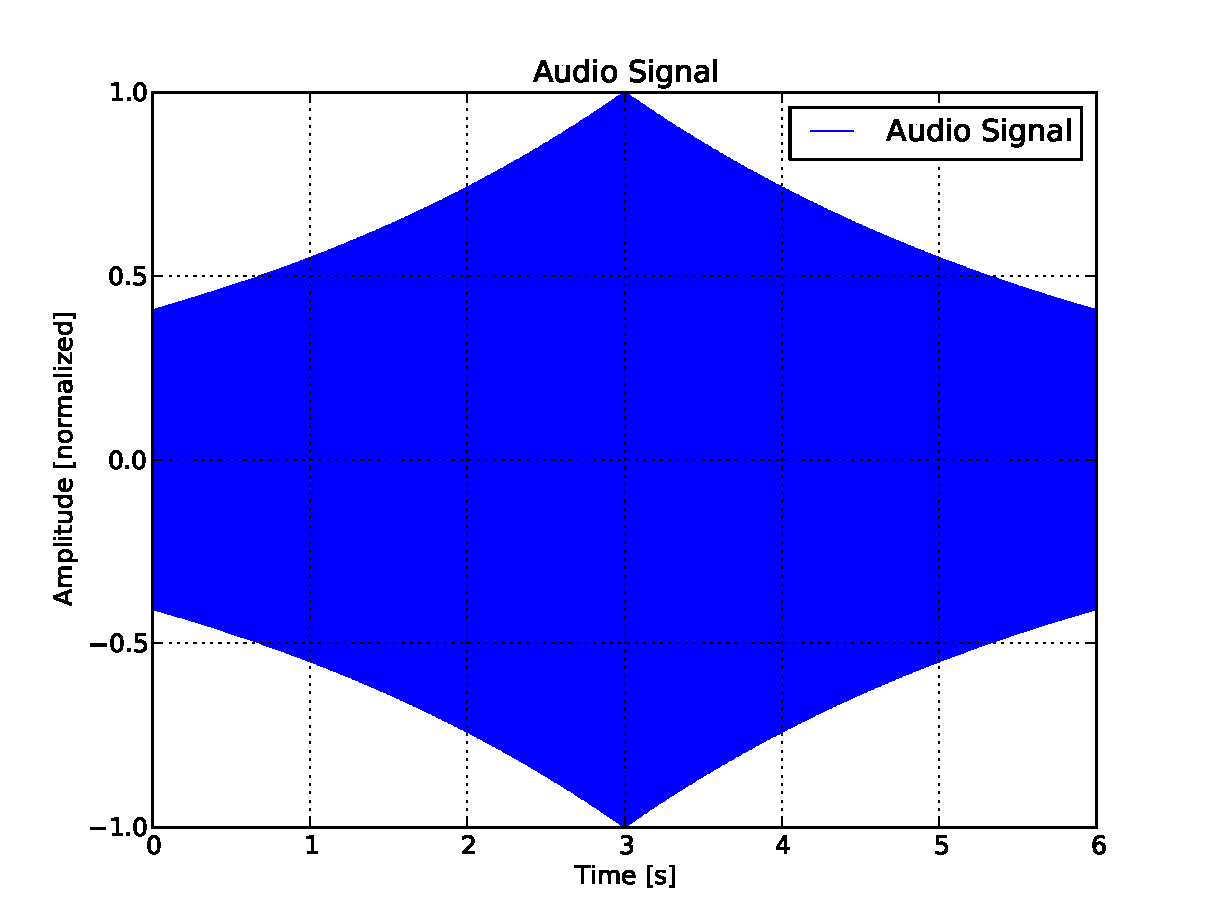
\includegraphics[width=0.90\textwidth]
	{./pictures/demo3_02.pdf}

	\caption{\small{Señal medida por el observador.}}
	
	\label{fig:doppler_audio}
\end{figure}
%.........................................................................


A continuación se explica cada parte del código


%ccccccccccccccccccccccccccccccccccccccccccccccccccccccccccccccccccccccccc
%DEMO 3_02
\begin{listing}[style=python, numbers = none]
import AudioLib as ad
\end{listing}
%ccccccccccccccccccccccccccccccccccccccccccccccccccccccccccccccccccccccccc
Se importa el mask para el manejo de \pyaudio, el archivo \texttt{AudioLib.py}
puede ser descargado de la página del curso\footnote{\url{https://github.com/sbustamante/Computacional-OscilacionesOndas/tree/master/codigos}}.

\
%ccccccccccccccccccccccccccccccccccccccccccccccccccccccccccccccccccccccccc
%DEMO 3_02
\begin{listing}[style=python, numbers = none]
#Velocidad del sonido [m/s]
vs = 331.5

#Creando objeto de audio
sonido = ad.audio()

#Intervalo de tiempo
dt = 1/(44100.)
#Frecuencia de nota [Hz]
freq0 = 110.

#Tiempo maximo	[s]
tmax = 6.
#Arreglo de tiempo
tiempo = np.arange( 0, tmax, dt )
#Nota a reproducir
nota = ad.Amplitude*np.sin( 2*np.pi*freq0*tiempo )

#Cargando nota de audio
sonido.load( nota )
#Reproduciendo sonido
sonido.play()
\end{listing}
%ccccccccccccccccccccccccccccccccccccccccccccccccccccccccccccccccccccccccc
En esta parte se define la velocidad del sonido en el aire como 
\texttt{vs = 331.5}. Luego se crea un objeto tipo audio, en el cual será 
almacenada la señal asociada al marco de referencia dela fuente. El intervalo
de tiempo \texttt{dt} se da en términos de la frecuencia $44100$ Hz, la cual
es un estándar para archivos de audio (Calidad CD)\footnote{Un valor inferior
produce una calidad de sonido peor. Ver \url{http://en.wikipedia.org/wiki/44,100_Hz}}

\

Se define la frecuencia original de la nota monofónica respecto al marco
de la fuente, en este caso \texttt{freq0 = 110.}, correspondiente a 
una nota \textit{La2}. Luego se da el tiempo máximo de muestreo del audio,
en segundos, \texttt{tmax = 6.} y se define el arreglo de tiempos como
\texttt{tiempo = np.arange( 0, tmax, dt )}.

\

En la siguiente línea se define la nota monofónica como \texttt{nota = 
ad.Amplitude}
\texttt{*np.sin( 2*np.pi*freq0*tiempo )}, donde \texttt{ad.Amplitude}
corresponde a la máxima amplitud que puede ser guardada en un archivo 
de audio \footnote{Las unidades de \texttt{ad.Amplitude} no están 
relacionadas con unidades físicas, es solo un formato de datos que 
determina la máxima posible amplitud almacenada.}. Finalmente, usando
el método \texttt{load} de la clase tipo audio, se carga esta nota en el
objeto de audio creado inicialmente \texttt{sonido.load( nota )} y se 
reproduce \texttt{sonido.play()}.

\
%ccccccccccccccccccccccccccccccccccccccccccccccccccccccccccccccccccccccccc
%DEMO 3_02
\begin{listing}[style=python, numbers = none]
#EFECTO DOPPLER ===========================================
#Creando objeto de audio asociado al observador
sonido_doppler = ad.audio()

#Distancia del observador a la carretera [m]
Lo = 1.0
#Velocidad del carro [m/s]
v_car = 6.0
#Distancia del carro inicialmente [m]
d_car = 18.0
#Tiempo de efecto doppler [s]
tmaxD = 6.0
#Arreglo de tiempo
tiempoD = np.arange( 0, tmaxD, dt )
#Numero de intervalos
Nt = int(len(tiempoD)/2.)
\end{listing}
%ccccccccccccccccccccccccccccccccccccccccccccccccccccccccccccccccccccccccc
De forma análoga al primer objeto, se crea el objeto de audio para 
almacenar la señal percibida por el observador \texttt{sonido\_doppler = 
ad.audio()}. A continuación se definen los parámetros físicos de la fuente
respecto al observador, esto es: \texttt{Lo = 1.0} la distancia en metros
del observador a la carretera, \texttt{v\_car = 6.0} la velocidad constante
del automóvil, en m/s, \texttt{d\_car = 18.0} la distancia inicial en metros 
entre el automóvil y el observador, y finamente el tiempo de muestreo en 
segundos \texttt{tmaxD = 6.0}, el arreglo de tiempo \texttt{tiempoD = 
np.arange( 0, tmaxD, dt )} y la mitad del número de intervalos de tiempo
\texttt{Nt = int(len(tiempoD)/2.)}.

\
%ccccccccccccccccccccccccccccccccccccccccccccccccccccccccccccccccccccccccc
%DEMO 3_02
\begin{listing}[style=python, numbers = none]
#Funcion de posicion del carro
def pos( t ):
    return -d_car + v_car*t
    
#Funcion de velocidad del carro dirigida a la fuente
def vel( t ):
    return v_car*1/np.sqrt( 1 + Lo**2/pos(t)**2 )
    
#Funcion de decaimiento de intensidad
def I( d ):
    return ad.Amplitude*np.exp(-abs(d)/20.)
    
#Transformacion de frecuencia Dopple
def freq( freq0, v, cond ):
    if cond == "Aleja":
	return freq0*vs/(vs - v)
    if cond == "Acerca":
	return freq0*vs/(vs + v)
\end{listing}
%ccccccccccccccccccccccccccccccccccccccccccccccccccccccccccccccccccccccccc
En esta parte del código se definen diferentes funciones para el cálculo
del efecto doppler. La función \texttt{pos( t )} determina la posición del
automóvil en función del tiempo respecto al observador, \texttt{I( d )}
da el decaimiento de la intensidad en función de la distancia y 
\texttt{freq( freq0, v, cond )}, donde \texttt{freq0} es la frecuencia 
original, \texttt{v} la velocidad relativa entre fuente y observador y 
\texttt{cond} puede tomar los valores de \texttt{'Aleja'} o \texttt{'Acerca'}
en función de la situación física que se presente.


\
%ccccccccccccccccccccccccccccccccccccccccccccccccccccccccccccccccccccccccc
%DEMO 3_02
\begin{listing}[style=python, numbers = none]
#Calculo de efecto Doppler para la nota inicial
notaD = np.zeros( 2*Nt )
#Cuando la fuente se acerca
notaD[:Nt] = I( pos(tiempoD[:Nt]) )*\
np.sin( 2*np.pi*freq(freq0, vel( tiempoD[:Nt] ), 'Acerca')*tiempoD[:Nt] )
#Cuando la fuente se aleja
notaD[Nt:] = I( pos(tiempoD[Nt:]) )*\
np.sin( 2*np.pi*freq(freq0, vel( tiempoD[Nt:] ), 'Aleja')*tiempoD[Nt:] )

#Cargando nota de audio
sonido_doppler.load( notaD )
#Reproduciendo sonido
sonido_doppler.play()
#Graficando Sonido
sonido_doppler.plot()
\end{listing}
%ccccccccccccccccccccccccccccccccccccccccccccccccccccccccccccccccccccccccc
Se crea un arreglo un arreglo para almacenar la señal en el marco de 
referencia del observador y posteriormente se calculan las dos contribuciones,
inicialmente cuando el automóvil de acerca \texttt{notaD[:Nt] = 
I( pos(tiempoD[:Nt]) )} \texttt{*np.sin( 2*np.pi*freq(freq0, vel( tiempoD[:Nt]),}

\texttt{'Acerca')*tiempoD[:Nt] )}, y cuando se aleja \texttt{notaD[Nt:] = }

\texttt{I( pos(tiempoD[Nt:]) )*np.sin( 2*np.pi*freq(freq0,} 

\texttt{vel( tiempoD[Nt:] ), 'Aleja')*tiempoD[Nt:] )}. Finalmente se carga
la señal al objeto de audio, se reproduce y se grafica.

%*************************************************************************